\section{Disruptor}
\label{sec:disruptor}

\nemquote{%
Death is the great disruptor. It thrusts us opposite life's mirror, invites our truthful exploration, and reveals the naked truth from which rebirth is possible and we are free to reinvent ourselves anew.
}{B.G. Bowers}

\nemchapterfirstletter{O}{ne} main goal of \codenamespace is to achieve high throughput.
In order to help achieve this goal, the disruptor\footnote{ \url{https://en.wikipedia.org/wiki/Disruptor_(software)} } pattern is used to perform most data processing.
A disruptor uses a ring buffer data structure to hold all elements in need of processing.
New elements are inserted into the next free slot of the ring buffer.
Fully processed elements are removed to make space for new elements.
Since the ring buffer has a finite number of slots, it can run out of space if processing can't keep up with new insertions.
The behavior of \codename, in such a case, can be configured to either to exit the server or discard new data until a slot becomes available.

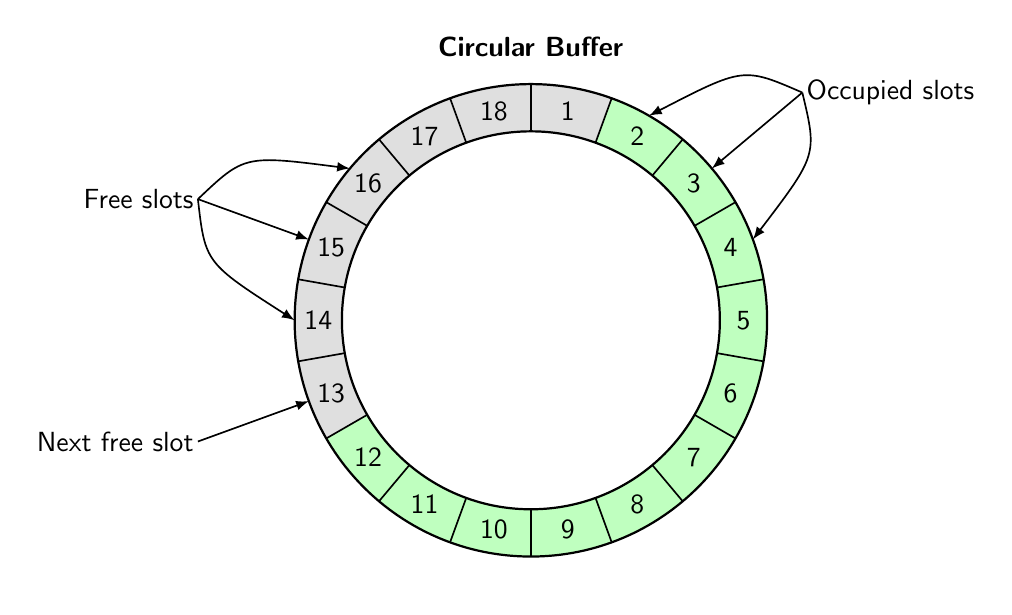
\begin{tikzpicture}[>=latex,font=\sffamily,semithick,scale=3,label distance=-2mm]
	\fill [green!25] (0,0) -- (70:1) arc [end angle=-150, start angle=70, radius=1] -- cycle;
	\fill [gray!25] (0,0) -- (70:1) arc [end angle=210, start angle=70, radius=1] -- cycle;
	\draw [thick,minimum size=6cm] (0,0) circle(1);
	\draw (90:1.1) node[label=above:\textbf{Circular Buffer}]{};
	\foreach \angle in {90,70,...,-70}
		\draw (\angle:1) -- (\angle-180:1);

	\foreach \angle [count=\anglei] in {80,60,...,-260}
		\draw (\angle:0.9) node[] {\anglei};

	\draw [thick,fill=white,minimum size=3cm] (0,0) circle(0.8);

	\draw [->] (160:1.5) .. controls (170:1.4) .. (180:1);
	\draw [->] (160:1.5) -- (160:1);
	\draw [->] (160:1.5) .. controls (150:1.4) .. (140:1);
	\draw [] (160:1.5) node[label=left:Free slots]{};

	\draw [->] (40:1.5) .. controls (50:1.4) .. (60:1);
	\draw [->] (40:1.5) -- (40:1);
	\draw [->] (40:1.5) .. controls (30:1.4) .. (20:1);
	\draw [] (40:1.5) node[label=right:Occupied slots]{};

	\draw [->] (200:1.5) -- (200:1);
	\draw (200:1.5) node[label=left:Next free slot]{};

	(Head.west);
\end{tikzpicture}

Each element in the ring buffer is processed by one or more consumers.
Each consumer takes a single element as input.
Some consumers calculate data from the input and attach it to the element, while others validate the element or alter the global chain state using the element's data.
Some consumers depend on the work done by previous consumers.
Therefore, consumers always need to act on input elements in a predefined order.
To ensure this, each consumer has an associated barrier.
The barrier prevents a consumer from processing an element that has not yet been processed by its immediately preceding consumer.
The last consumer reclaims all memory that was used during processing.
Consumers can set an element's completion status to \structField{CompletionStatus}{Aborted} in case it is already known or invalid for some reason.
Subsequent consumers ignore aborted elements.

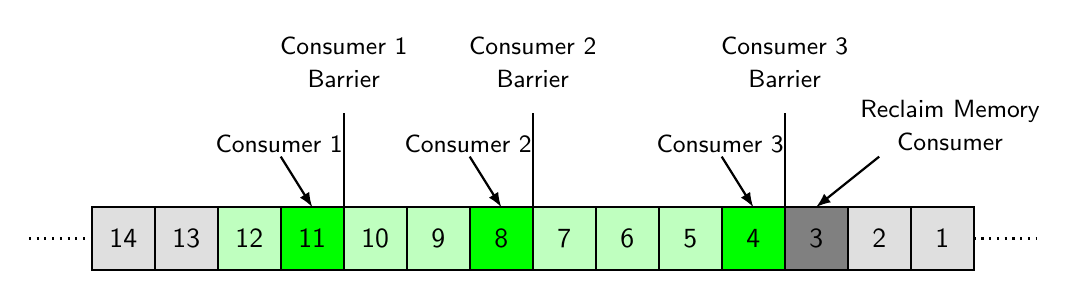
\begin{tikzpicture}[>=latex,font=\sffamily,thick,,scale=0.8]
	% Dots
	\draw[thick,dotted,step=.5] (0,0.5) grid (1,0.5);
	\draw[thick,dotted,step=.5] (15,0.5) grid (16,0.5);

	% Rectangles
	\foreach \i [] in {1,2,13,14}
		\filldraw[draw=black,fill=gray!25] (\i,0) rectangle (\i+1,1);
	\foreach \i [] in {3,5,6,8,9,10}
		\filldraw[draw=black,fill=green!25] (\i,0) rectangle (\i+1,1);
	\foreach \i [] in {4,7,11}
		\filldraw[draw=black,fill=green] (\i,0) rectangle (\i+1,1);
	\filldraw[draw=black,fill=gray] (12,0) rectangle (13,1);

	% Consumer 1
	\draw [] (5,2.0) node[xshift=0.25cm,label=left:\small{Consumer 1}]{};
	\draw [->] (4,1.8) -- (4.5,1);
	\draw [] (5,3.3) node[align=center]{\small{Consumer 1}\\\small{Barrier}};
	\draw [] (5,1) -- (5, 2.5);

	% Consumer 2
	\draw [] (8,2.0) node[xshift=0.25cm,label=left:\small{Consumer 2}]{};
	\draw [->] (7,1.8) -- (7.5,1);
	\draw [] (8,3.3) node[align=center]{\small{Consumer 2}\\\small{Barrier}};
	\draw [] (8,1) -- (8, 2.5);

	% Consumer 3
	\draw [] (12,2.0) node[xshift=0.25cm,label=left:\small{Consumer 3}]{};
	\draw [->] (11,1.8) -- (11.5,1);
	\draw [] (12,3.3) node[align=center]{\small{Consumer 3}\\\small{Barrier}};
	\draw [] (12,1) -- (12, 2.5);

	% Reclaim memory consumer
	\draw [] (13,2.3) node[align=center,xshift=1.3cm]{\small{Reclaim Memory}\\\small{Consumer}};
	\draw [->] (13.5,1.8) -- (12.5,1);

	% Numbers
	\foreach \index [count=\indexi] in {14,13,...,1}
		\draw (\indexi+0.5,0.5) node[] {\index};
\end{tikzpicture}

\subsection{Consumers}
\index{consumers}
\label{sec:disruptor:consumers}
In \codename, a block disruptor is used to process incoming blocks and blockchain parts.
A blockchain part is an input element composed of multiple blocks.
This disruptor is primarily responsible for validating, reconciling and growing the blockchain.

A transaction disruptor is used to process incoming, unconfirmed transactions.
Transactions that are fully processed get added to the unconfirmed transactions cache.

All disruptors are associated with a chain of consumers that perform all processing of their input elements.
Different disruptors are customized by using different consumer chains.
All consumers can inspect the data being processed and some can modify it.

\begin{figure}[H]
	\nemcenterwithcaption{
		\begin{subfigure}{.5\textwidth}
			\nemcenterwithcaption{
				\tikzstyle{consumer} = [rectangle, rounded corners, text centered, draw=black, minimum width=7cm, minimum height=0.5cm, text width=6.5cm]
				\vspace{0pt}
				\begin{tikzpicture}[>=latex,font=\small ,semithick,scale=1,node distance=1.1cm]
					% block consumers
					\node (audit consumer) [consumer] {Audit Consumer (optional)};
					\node (hash calculator consumer) [consumer, below of=audit consumer] {Hash Calculator Consumer};
					\node (hash check consumer) [consumer, below of=hash calculator consumer] {Hash Check Consumer};
					\node (blockchain check consumer) [consumer, below of=hash check consumer] {Blockchain Check Consumer};
					\node (stateless validation consumer) [consumer, below of=blockchain check consumer] {Stateless Validation Consumer};
					\node (batch signature consumer) [consumer, below of=stateless validation consumer] {Batch Signature Consumer};
					\node (blockchain sync consumer) [consumer, below of=batch signature consumer] {Blockchain Sync Consumer};
					\node (blockchain sync cleanup consumer) [consumer, below of=blockchain sync consumer] {Blockchain Sync Cleanup Consumer (optional)};
					\node (new block consumer) [consumer, below of=blockchain sync cleanup consumer] {New Block Consumer};

					% arrows
					\draw [semithick,->] (audit consumer) -- (hash calculator consumer);
					\draw [semithick,->] (hash calculator consumer) -- (hash check consumer);
					\draw [semithick,->] (hash check consumer) -- (blockchain check consumer);
					\draw [semithick,->] (blockchain check consumer) -- (stateless validation consumer);
					\draw [semithick,->] (stateless validation consumer) -- (batch signature consumer);
					\draw [semithick,->] (batch signature consumer) -- (blockchain sync consumer);
					\draw [semithick,->] (blockchain sync consumer) -- (blockchain sync cleanup consumer);
					\draw [semithick,->] (blockchain sync cleanup consumer) -- (new block consumer);
				\end{tikzpicture}
			}{Block Consumers}
		\end{subfigure}%
		\begin{subfigure}{.5\textwidth}
			\nemcenterwithcaption{
				\tikzstyle{consumer} = [rectangle, rounded corners, text centered, draw=black, minimum width=6cm, minimum height=0.6cm, text width=6.5cm]
				\vspace{0pt}
				\begin{tikzpicture}[>=latex,font=\small,semithick,scale=1,node distance=1.1cm]
					% transactions consumers
					\node (audit consumer) [consumer] {Audit Consumer (optional)};
					\node (hash calculator consumer) [consumer, below of=audit consumer] {Hash Calculator Consumer};
					\node (hash check consumer) [consumer, below of=hash calculator consumer] {Hash Check Consumer};
					\node (dummy1) [consumer, below of=hash check consumer, draw=none] {};
					\node (stateless validation consumer) [consumer, below of=dummy1] {Stateless Validation Consumer};
					\node (batch signature consumer) [consumer, below of=stateless validation consumer] {Batch Signature Consumer};
					\node (dummy2) [consumer, below of=batch signature consumer, draw=none] {};
					\node (dummy3) [consumer, below of=dummy2, draw=none] {};
					\node (new transactions consumer) [consumer, below of=dummy3] {New Transactions Consumer};

					% arrows
					\draw [semithick,->] (audit consumer) -- (hash calculator consumer);
					\draw [semithick,->] (hash calculator consumer) -- (hash check consumer);
					\draw [semithick,->] (hash check consumer) -- (stateless validation consumer);
					\draw [semithick,->] (stateless validation consumer) -- (batch signature consumer);
					\draw [semithick,->] (batch signature consumer) -- (new transactions consumer);
				\end{tikzpicture}
			}{Transactions Consumers}
		\end{subfigure}
	}{\codenamespace consumer chains}
\end{figure}

\subsubsection{Common Consumers}
\label{sec:disruptor:commonConsumers}
\index{consumers!common}
The block and transaction disruptors share a number of consumers.

\subsubsection*{Audit Consumer}
This consumer is optional and can be enabled via node configuration.
If enabled, all new elements are written to disk.
This makes it possible to replay the incoming network action and is helpful for debugging.

\subsubsection*{Hash Calculator And Hash Check Consumers}
It is very common for a server to receive the same element many times because networks consist of many servers that broadcast elements to several other servers.
For performance reasons, it is desirable to detect at an early stage whether an element has already been processed in order to avoid processing it again.

The hash calculator consumer calculates all the hashes associated with an element.
The hash check consumer uses the hashes to search the recency cache, which contains the hashes of all recently seen elements.
The consumer used by the transaction disruptor will also search the hash cache (containing hashes of confirmed transactions) and the unconfirmed transactions cache.
If the hash is found in any cache, the element is marked as \structField{CompletionStatus}{Aborted} and further processing is bypassed.

\subsubsection*{Stateless Validation Consumer}
This consumer handles state independent validation by validating each entity in an element.
This can be done in parallel using many threads.
Each plugin can add stateless validators.

An example of a stateless validation is the validation that a block does not contain more transactions than allowed by the network.
This check depends on the network configuration but not on the global blockchain state.

\subsubsection*{Batch Signature Consumer}
This consumer validates all signatures of all entities in an element.
This is separate from the \emph{Stateless Validation Consumer} because it uses batch verification.
For improved performance, this consumer processes many signatures at once in a batch instead of individually.
This can be done in parallel using many threads.

\subsubsection*{Reclaim Memory Consumer}
This consumer completes processing of and frees all memory associated with an element.
It triggers downstream propagation of the statuses of all transactions that were updated during processing.
The overall result of the sync operation is used to update the reputation of - and possibly ban - the sync partner \nemrefparens{sec:reputation}).

\subsubsection{Additional Block Consumers}
\label{sec:disruptor:blockConsumers}
\index{consumers!block}
The block disruptor also uses a few block-specific consumers.

\subsubsection*{Blockchain Check Consumer}
This consumer performs state-independent integrity checks of the chain part contained within an element.
It checks that:
\begin{itemize}
	\item The chain part is not composed of too many blocks.
	\item The timestamp of the last block in the chain part is not too far in the future.
	\item All blocks within the chain part are linked.
	\item There are no duplicate transactions within the chain part.
\end{itemize}

\subsubsection*{Blockchain Sync Consumer}
This consumer is the most complex one.
All tasks that require or alter the local server's chain state are performed in this consumer.

First, it checks that the new chain part can be attached to the existing chain.
If the chain part attaches to a block preceding the tail block, all blocks starting with the tail block are undone in reverse order until the common block is reached.

Next, it executes each block by performing stateful validation and then observing changes.
Stateless validation is skipped because it was performed by previous consumers.
If there are any validation failures, the entire chain part is rejected.
Otherwise, all changes are committed to the chain state (both the block and cache storages) and the unconfirmed transactions cache is updated.

\emph{This consumer is the only part of the \codenamespace system that modifies the chain state and needs write access to it.}

\subsubsection*{Blockchain Sync Cleanup Consumer}
This consumer is optional and can be enabled via node configuration.
If enabled, it removes all files that were created by the \emph{Blockchain Sync Consumer}.
This consumer should only be enabled when a server is running without a broker.

\subsubsection*{New Block Consumer}
This consumer forwards single blocks, either harvested by the server or pushed from a remote server, to other servers in the network.

\subsubsection{Additional Transaction Consumers}
\label{sec:disruptor:transactionConsumers}
\index{consumers!transaction}
The transaction disruptor uses a single transaction-specific consumer.

\subsubsection*{New Transactions Consumer}
This consumer forwards all transactions that have valid signatures and have passed stateless validation to the network.
Stateful validation is not performed on transactions until they're added to the unconfirmed transactions cache.
Forwarding is intentionally done before stateful validation because one server might reject transactions that could be accepted by other servers (e.g. if the transaction has too low a fee for the local server).
Subsequently, stateful validation is performed on the forwarded transactions, and the valid ones are stored in the unconfirmed transactions cache.
